\chapter{Redes de interacción entre tortugas}
\graphicspath{{figs/}}

\chapterquote{In retrospect, Euler's unintended message is very simple: Graphs or networks have properties, hidden in their construction, that limit or enhance our ability to do things with them.}{Albert-László Barabási, 1982}

\label{Redes de interacción entre tortugas}
\section{Trayectorias }

Primero se muestran las trayectorias obtenidas para un día de medición (Fig.~\ref{fig:trayeSinFiltr}), como por ejemplo 1/12/2020. Para éstas se realizó un programa en el lenguaje Python utilizando la librería Folium, permitiendo añadir puntos de GPS al mapa \cite{github}.
 
\begin{figure}[h]
    \begin{center}
       
   
    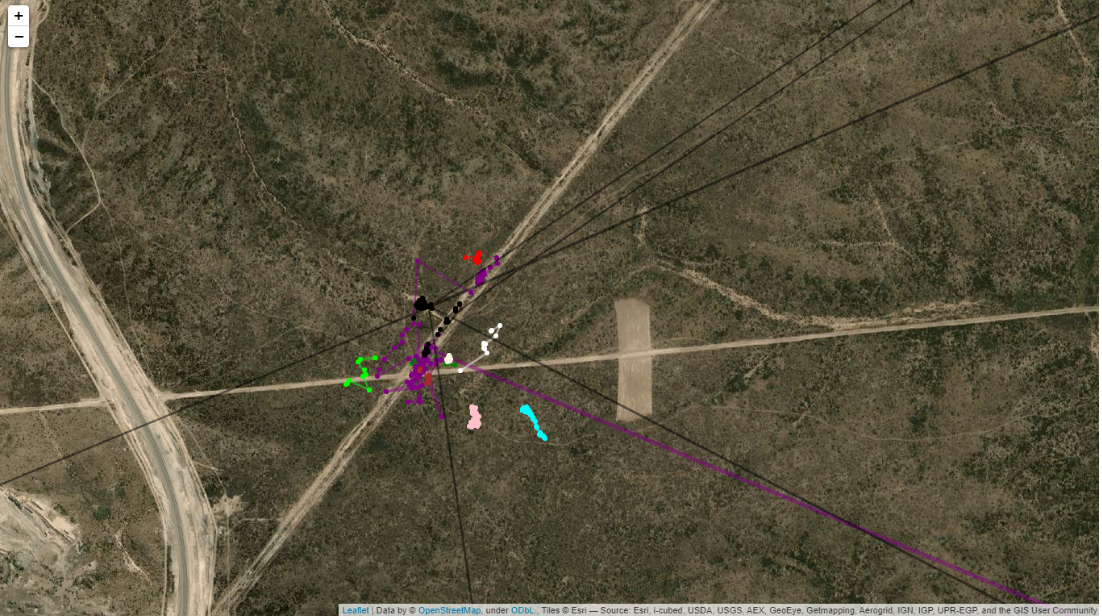
\includegraphics[width=\imsize]{Chap2/Traye1_12_sinF.png}
\end{center}
    \caption[Trayectorias un dia de medición, sin filtrrar.]{Trayectorias del 1/12/2020, cada color representa una tortuga diferente. Ambas metodologías fueron implementadas, algunos puntos tomados con el tortugómetro escapan a la trayectoria esperada.}
    \label{fig:trayeSinFiltr}
\end{figure}
Se observa en la Fig.~\ref{fig:trayeSinFiltr}, que algunos puntos tomados por el tortugómetro se desvían de la trayectoria esperada para una tortuga (recorren distancias del orden de los kilómetros en menos de 10 minutos). Se estima que estas desviaciones se producen por dos motivos: en primer lugar, en los primeros minutos de medición, el GPS comienza a conectarse a satélites hasta tener la precisión máxima, haciendo que  los primeros puntos tengan una mayor desviación; en segundo lugar, se observó de manera aleatoria la desviación de algún punto respecto de la trayectoria típica.
 
 
 
 
Para corregir estas desviaciones, se implementó un método basado en la velocidad máxima que pueden alcanzar los individuos. El mismo está detallado en el repositorio de GitHub, archivo \textit{CriterioParaSacarData.py} \cite{github}. Para obtener la velocidad máxima, se calculó la distribución de velocidades de la Fig.~\ref{fig:distribuciondeVel}.

 
\begin{figure}[h]
\begin{center}
       
   
    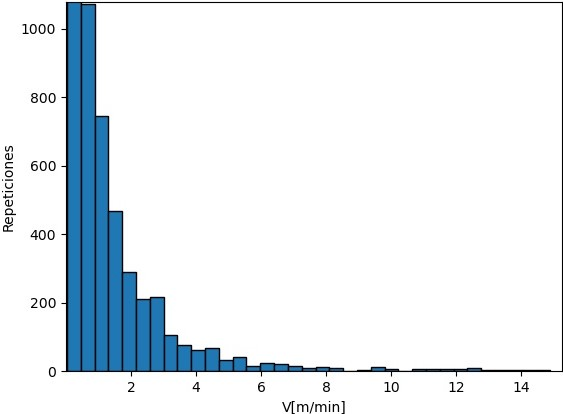
\includegraphics[width=\imsize]{Chap2/Velocidades2.jpeg}
    \caption[Distribución de velocidades.]{Histograma de velocidades en m/min. Las  velocidades obtenidas mayores a 15 m/min están órdenes de magnitud por encima.}
    \label{fig:distribuciondeVel}
\end{center}
\end{figure}
Se observó en la distribución de velocidades de la Fig.~\ref{fig:distribuciondeVel}, que las tortugas llegan a una velocidad máxima de aproximadamente 15m/min, de manera que se adoptó el criterio de filtrar los tramos de trayectoria en los que la velocidad supera ese valor máximo. Filtrando los puntos de la Fig.~\ref{fig:trayeSinFiltr}, tomando velocidad máxima 15 m/min, se obtuvo  el mapa de la Fig.~\ref{fig:trayeConFiltr}.
 
 
 

\begin{figure}[h]
    \begin{center}
       
   
    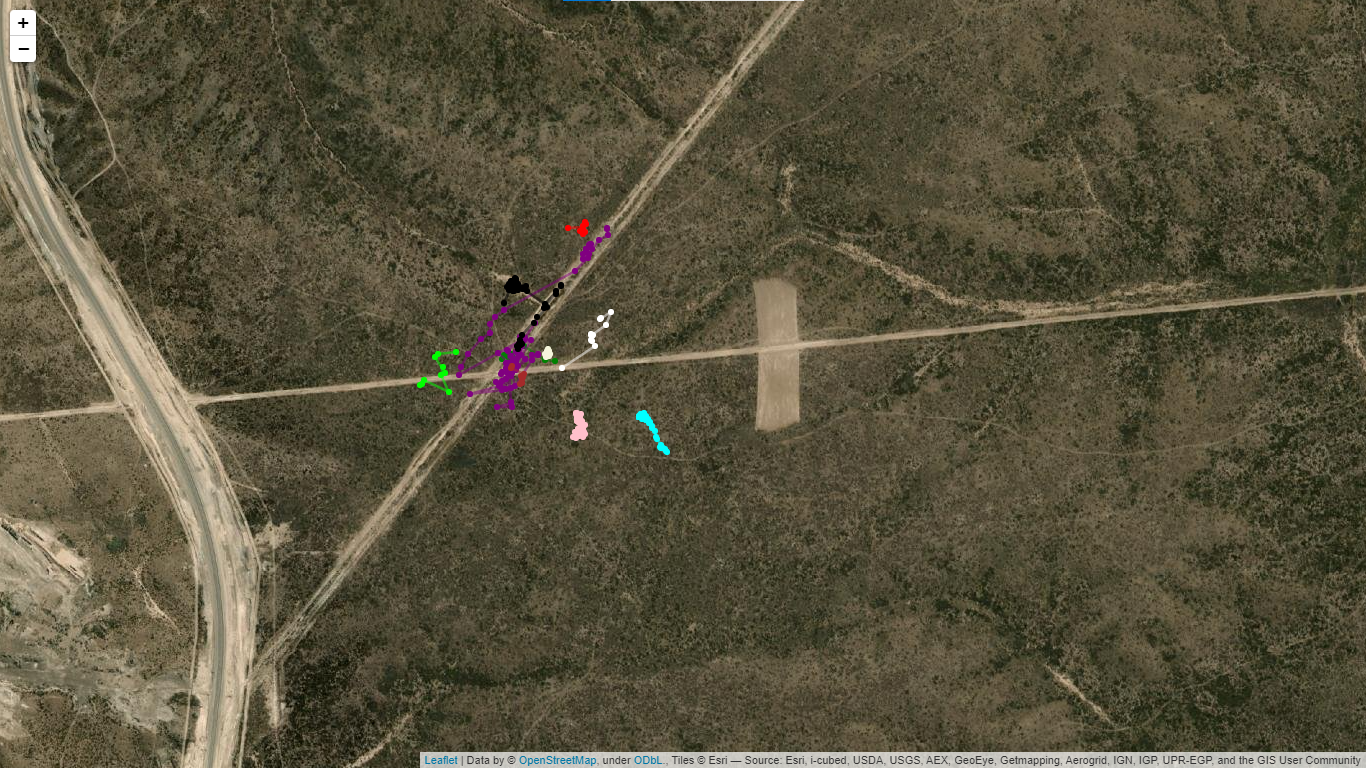
\includegraphics[width=\imsize]{Chap2/Traye1_12_conF.png}
\end{center}
    \caption[Trayectorias un dia de medición, despues del filtrado.]{Trayectorias del 1/12/2020 luego del filtrado, cada color representa una tortuga diferente.}
    \label{fig:trayeConFiltr}
\end{figure}

\section{Red de encuentros}
Partiendo de las trayectorias filtradas, se decidió buscar el solapamiento de las trayectorias, para identificar los encuentros. Para ello, se implementó un codigo en Python, que partiendo de cualquier punto de su trayectoria busca si hay otro punto de otra tortuga que se encuentre a una distancia menor a 20 metros y a una distancia temporal menor a 20 minutos. Cuando se cumple esta condición se van guardando los pares de puntos junto con la hora y el nombre de ambas tortugas. 

Utilizando los encuentros calculados, se armaron dos redes de interacción  en la librería NetworkX \cite{networkx}, una para los datos obtenidos utilizando  tortugometro y otra para los datos provenientes de i-gotU (\ref{fig:redInteraccion20mincampanas} y otra). Las conexiones entre nodos tortugas tienen peso linealmente dependiente de la cantidad de encuentros entre ellas, esto se observa en el grosor del link entre dos tortugas y las distancias relativas entre nodos.


\begin{figure}[h]
    \begin{center}
       
   
    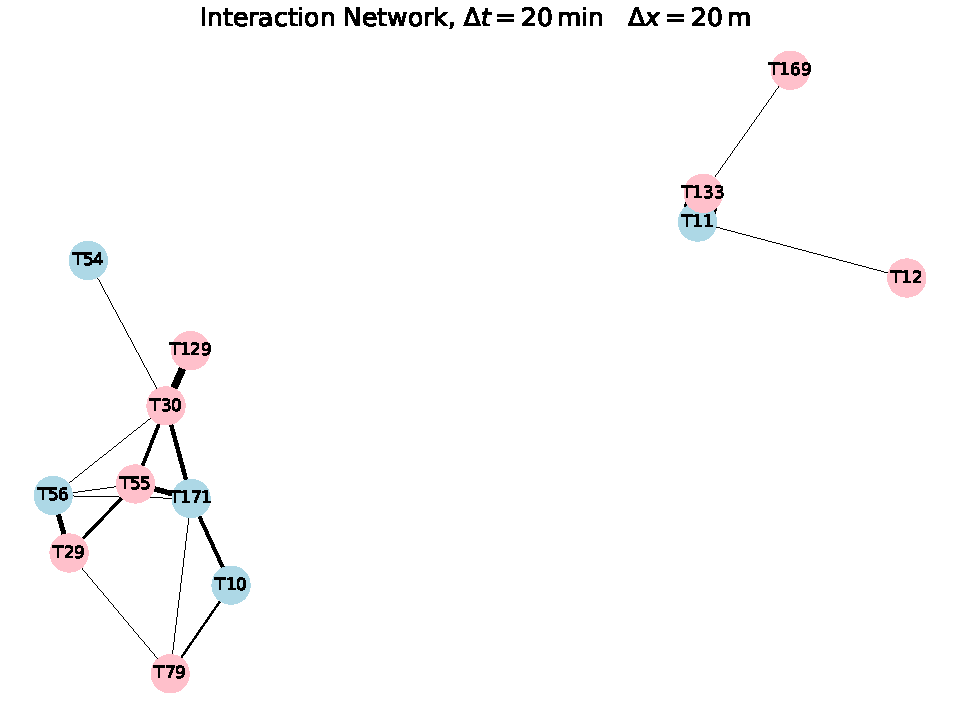
\includegraphics[width=\imsize]{Chap2/red_interaccion_20min_campanas.pdf}
\end{center}
    \caption[Red de encuentros entre tortugas utilizando telemetria y tortugometro.]{Red de encuentros entre tortugas para datos provenientes de las metodologías telemetria y tortugometro. La condición de encuentro esta dada por una distancia espacial menor a 20 metros y a una distancia temporal menor a 20 minutos.}
    \label{fig:redInteraccion20mincampanas}
\end{figure}



\begin{figure}[h]
    \begin{center}
       
   
    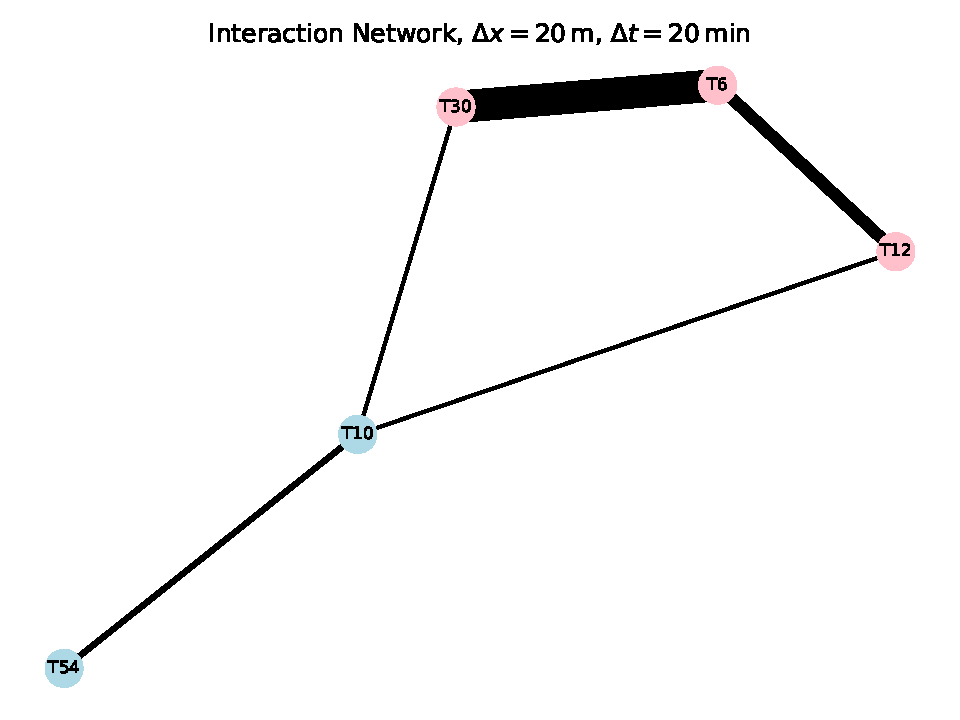
\includegraphics[width=\imsize]{Chap2/red_interaccion_20min_IGOTO.pdf}
\end{center}
    \caption[Red de encuentros entre tortugas utilizando i-gotU.]{Red de encuentros entre tortugas para datos provenientes de las metodologías i-gotU. La condición de encuentro esta dada por una distancia espacial menor a 20 metros y a una distancia temporal menor a 20 minutos.}
    \label{fig:redInteraccion20igotu}
\end{figure}


\begin{Huge}
Idea : conectar con criterio de encuentros mostrar grafico de encuentros segun la epoca del año y pasar a las dos redes de interacción que tenemos 
\end{Huge}

%%% Local Variables: 
%%% mode: latex
%%% TeX-master: "template"
%%% End: 
